\documentclass{article}
\usepackage[utf8]{inputenc}
\usepackage{graphicx}
\usepackage[margin=1in]{geometry}
\usepackage{float}
\usepackage{amsmath}
\usepackage{epstopdf}
\usepackage{wrapfig}

\title{Final Project- Tunable Ring Oscillator}
\author{Dan Kearney and Theo Thompson}
\date{May 9, 2013}

\begin{document}
\maketitle

\section*{Prelab}
Talk about mathematical analysis, ``turn on power'' analysis, time constants, in general what the starver does, etc.\\
Talk about simulation results yolo\\
mention the many everyday application sof a ring oscillator

\section*{Simulation Results}

\begin{figure}[H]
\centering
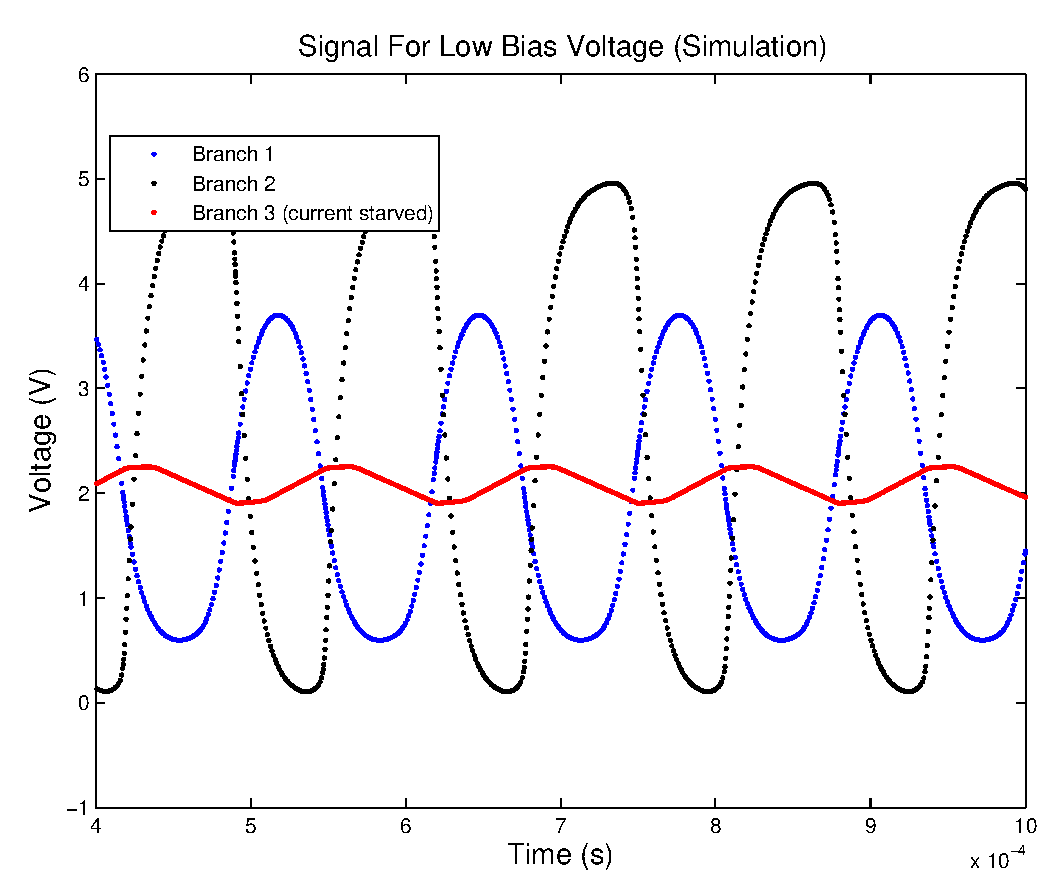
\includegraphics[scale=1]{lowBiasSigSim.eps}
\caption{}
\label{lowBiasSim}
\end{figure}

\begin{figure}[H]
\centering
\includegraphics[scale=1]{highBiasSigSim.eps}
\caption{}
\label{highBiasSim}
\end{figure}

\begin{figure}[H]
\centering
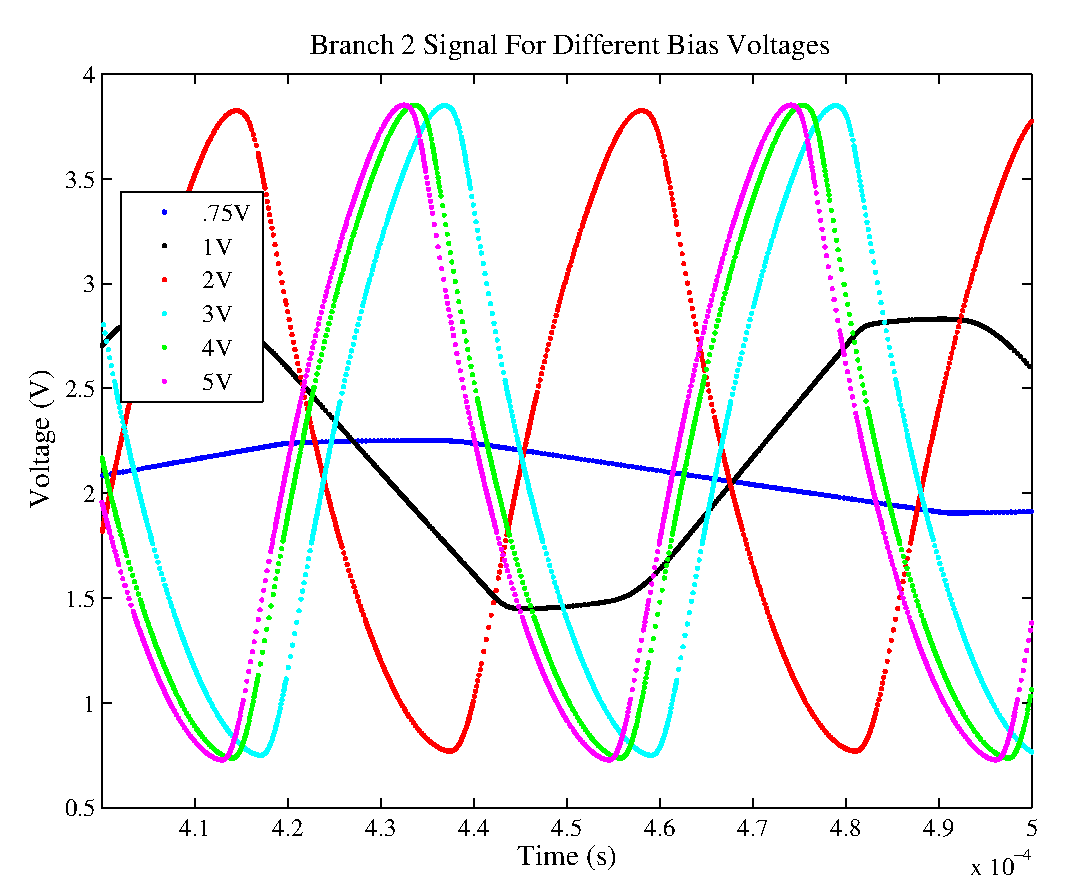
\includegraphics[scale=1]{branch2DiffBiasSim.eps}
\caption{}
\label{branch2DiffBiasSim}
\end{figure}


\begin{figure}[H]
\centering
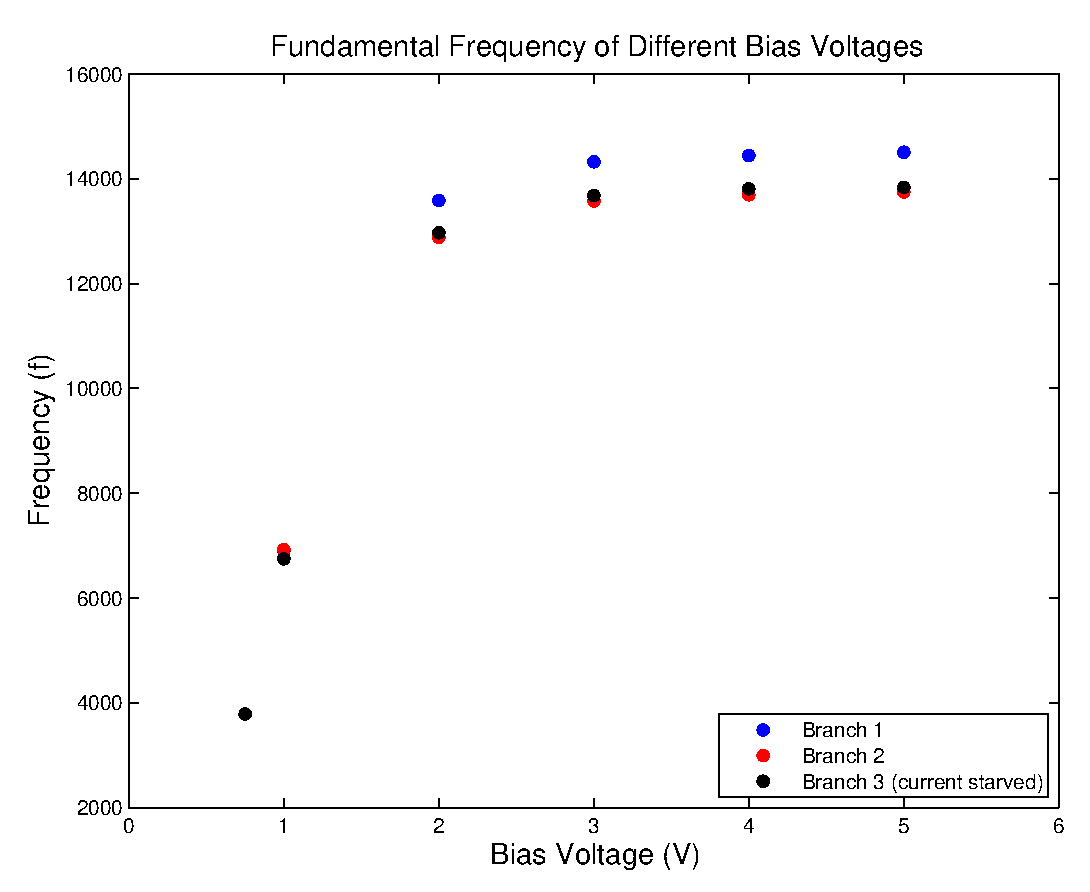
\includegraphics[scale=1]{biasFrequenciesSim.eps}
\caption{}
\label{biasFrequenciesSim}
\end{figure}

\section{Results}
talk about plots. maybe fit a theoretical to them.
plots:\\
signal for several bias voltages (same plot?)\\
signal for different branches\\
comparison to simulation results\\
frequency as a function of bias voltage\
\section{Postlab}
talk about stuff we didn't expect. why was one branch different? why do we exist? why driving a speaker doesn't make sense. Applications of our work. Which branch is the best if you are gonna make an oscillator? what should you do if you want frequencies above/below this range?

% \begin{figure}[H]
% \centering
% \includegraphics[scale=.7]{pinchungpoo}
% \caption{pinshungpoo}
% \label{schem}
% \end{figure}

\end{document}